\documentclass[11pt,italian]{article}
\usepackage[T1]{fontenc}
\usepackage[utf8]{inputenc} %utf8 % lettere accentate da tastiera
\usepackage[italian]{babel} % lingua del documento
\usepackage{blindtext}
\usepackage{enumitem}
\usepackage{float}
\usepackage{xcolor}   % for \textcolor
\usepackage[font=small,labelfont=bf,skip=10pt]{caption}
\usepackage{subcaption}
\setlength{\belowcaptionskip}{5pt}
\usepackage{listings}
\lstset{
  basicstyle=\ttfamily,
  columns=fullflexible,
  frame=single,
  breaklines=true,
  postbreak=\mbox{\textcolor{red}{$\hookrightarrow$}\space},
}
\usepackage{hyperref}
\usepackage{cleveref}
\usepackage{graphicx}
\graphicspath{ {./images/} }

% Use lstinline as item in description
\makeatletter
\newcommand*{\lstitem}[1][]{%
  \setbox0\hbox\bgroup
    \patchcmd{\lst@InlineM}{\@empty}{\@empty\egroup\item[\usebox0]\leavevmode\ignorespaces}{}{}%
    \lstinline[#1]%
}
\makeatother

\title{Multiple Sequence Alignment (MSA) \\ di sequenze SARS-CoV-2}

\date{A.A.: 2019/2020}

\author{
    \textsc{Edoardo Silva} 816560 \\
    \textsc{Davide Marchetti} 815990
}

\begin{document}
\maketitle

\section*{Abstract}
Il SARS-CoV-2 (dall'inglese \textit{Severe Acute Respiratory Syndrome CoronaVirus 2}), è un ceppo virale della specie SARS-related coronavirus/SARS-CoV, facente parte del genere Betacoronavirus (ceppo di virus a RNA).

Il virus è stato sequenziato genomicamente dopo un test di acido nucleico effettuato su un campione prelevato da un paziente colpito da una polmonite, di cui non si conosceva la causa, ad inizio Dicembre 2019 a Wuhan, città continentale a est della Cina.

L'obiettivo del progetto consiste nell'analizzare, allineare ed identificare le differenze con la sequenza di riferimento prelevata su un campione di Wuhan, progettando un formato di output nel quale memorizzare i risultati ottenuti.

Usando i sequenziamente genomici del virus denominato Covid-19, reperibili tramite NCBI\footnote{\url{https://www.ncbi.nlm.nih.gov/genbank/sars-cov-2-seqs/}} e GISAID\footnote{\url{https://www.gisaid.org/}} e sfruttando gli strumenti messi a disposizione dall'European Bioinformatics Institute\footnote{\url{https://www.ebi.ac.uk/Tools/msa/}} abbiamo effettuato l'allineamento di un insieme di sequenze relative a paesi del medioriente.

\newpage
\section{Sequenze Analizzate}
In aggiunta alla sequenza di riferimento di Wuhan, ne sono state selezionate alcune relative a paesi dell'area mediorientale.

\subsubsection*{Reference di Wuhan}
\begin{description}
    \lstitem{NC_045512.2} pubblicata il 17/01/2020 (ultimo aggiornamento)
\end{description}

\subsubsection*{Iran}
\begin{description}
    \lstitem{MT320891.2} pubblicata il 10/04/2020
    \lstitem{MT281530.2} pubblicata il 04/04/2020
    \lstitem{EPI_ISL_442523} sequenziata il 09/03/2020
    \lstitem{EPI_ISL_437512} sequenziata il 26/03/2020
\end{description}

\subsubsection*{Israele}
\begin{description}
    \lstitem{MT276598.1} sequenziata il 02/04/2020
    \lstitem{MT276597.1} sequenziata il 02/04/2020
    \lstitem{EPI_ISL_447469} sequenziata il 14/04/2020
\end{description}

\subsubsection*{Pakistan}
\begin{description}
    \lstitem{MT262993.1} pubblicata il 25/03/2020
    \lstitem{MT240479.1} pubblicata il 25/03/2020
    \lstitem{EPI_ISL_417444} sequenziata il 04/03/2020
\end{description}

\subsubsection*{Turchia}
\begin{description}
    \lstitem{MT327745.1} pubblicata il 13/04/2020,
    \lstitem{EPI_ISL_437334} sequenziata il 24/03/2020
    \lstitem{EPI_ISL_437317} sequenziata il 27/03/2020
\end{description}

\section{Strumenti utilizzati}
L'analisi è stata effettuata utilizzando \lstinline{Clustal Omega} e \lstinline{MUSCLE}, due strumenti per l'allineamento di sequenze multiple (MSA) accessibili attraverso un'interfaccia web\footnote{\url{https://www.ebi.ac.uk/Tools/msa/clustalo/}} \footnote{\url{https://www.ebi.ac.uk/Tools/msa/muscle/}}.

% \newpage
\section{Analisi preliminare}
\label{section:pre-analysis}
Una prima analisi delle sequenze è stata effettuata con l'ausilio di Jalview\footnote{\url{https://www.jalview.org/}}, un software open source che offre la possibilità di generare una visualizzazione grafica degli gli allineamenti effettuati dai tool.

\begin{figure}[H]
  \makebox[\textwidth][c]{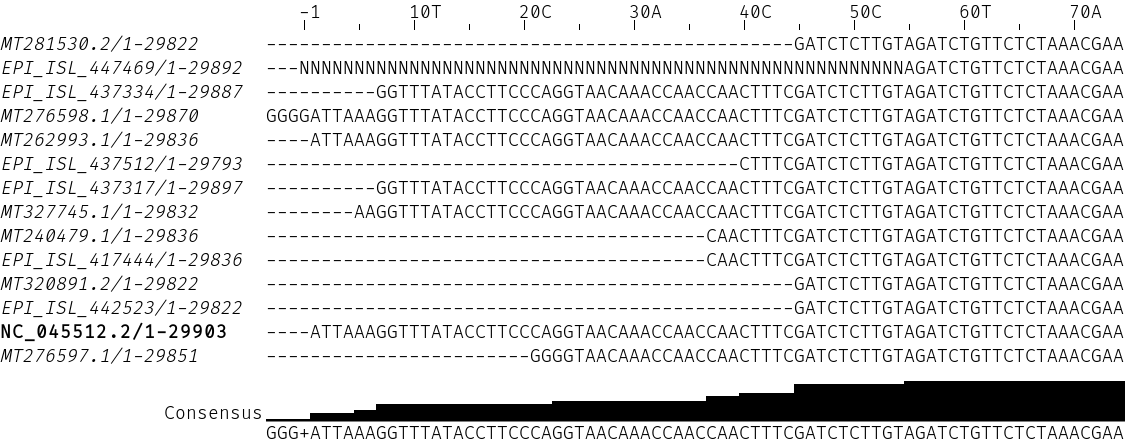
\includegraphics[width=1.3\linewidth]{jalview-clustal-start.png}}
  \caption{Differenze all'inizio dell'allineamento}
  \label{fig:jalview-start}
\end{figure}

Tramite questo strumento è possibile notare aspetti interessanti: esaminando l'allineamento la maggior parte delle differenze sono concentrate agli estremi dello stesso (\cref{fig:jalview-start,fig:jalview-end}).

\begin{figure}[H]
  \makebox[\textwidth][c]{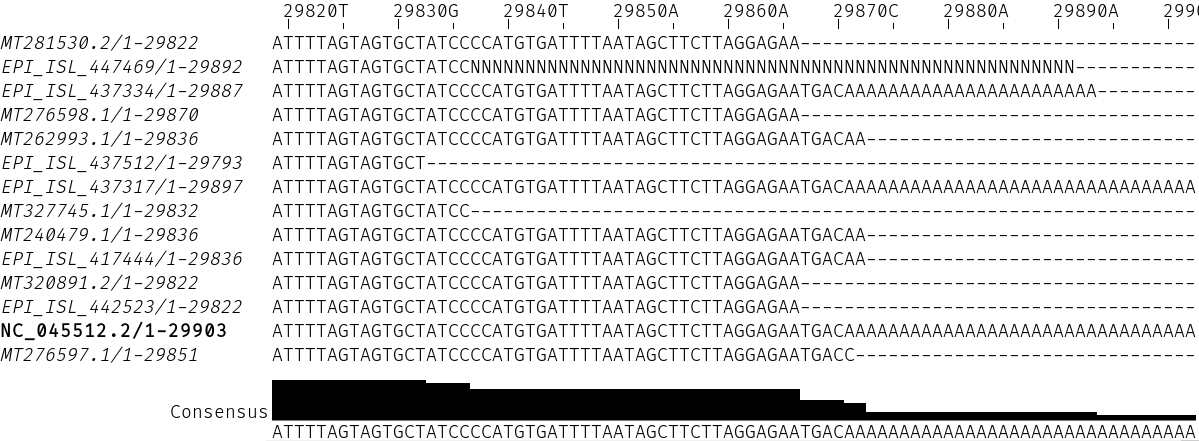
\includegraphics[width=1.3\linewidth]{jalview-clustal-end.png}}
  \caption{Differenze alla fine dell'allineamento}
  \label{fig:jalview-end}
\end{figure}

\vfill
Inoltre, due delle sequenze selezionate presentano basi mancanti o possibili problemi nel sequenziamento (\cref{fig:jalview-inner}).
Quest'ultimi verranno successivamente interpretate e considerate come match rispetto al reference qualora rispettino la codifica definita dallo IUPAC Code\footnote{\url{https://www.bioinformatics.org/sms/iupac.html}}.
\vfill

\begin{figure}[H]
  \makebox[\textwidth][c]{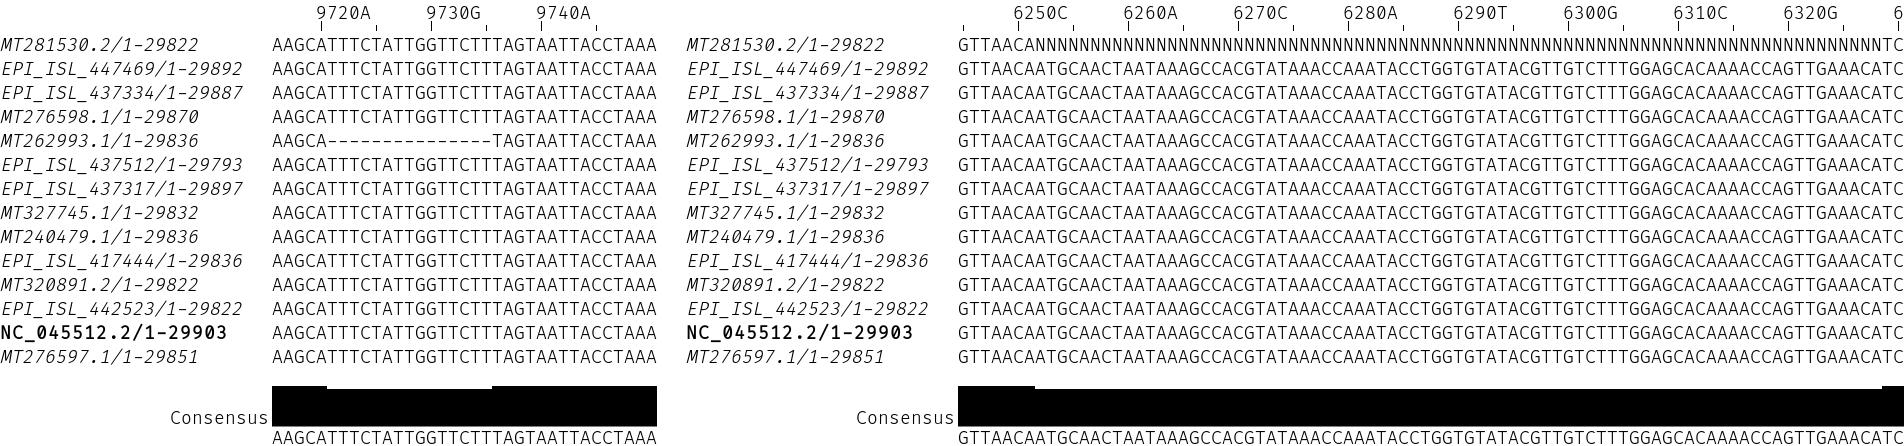
\includegraphics[width=1.5\linewidth]{jalview-clustal-inner.png}}
  \caption{Differenze all'interno delle sequenze}
  \label{fig:jalview-inner}
\end{figure}

\newpage
\section{Struttura del codice}
L'esecuzione dell'analisi prevede, per ogni file di allineamento fornito in input, un corrispondente file di output che raggruppa le regioni di non match delle sequenze analizzate.

\noindent
Lo script è composto da diversi file, ciascuno con la propria funzione specifica:
\begin{description}
  \lstitem{alignment_model.py:} definisce le strutture dati che verranno utilizzate dal parser per memorizzare i contenuti letti.
  \lstitem{matcher.py:} contiene la classe che identifica le regioni di match/mismatch.
  \lstitem{main.py:} entrypoint dello script che coordina l'esecuzione dell'analisi.
  \lstitem{parsers.py:} definisce una classe per ogni tool di allineamento utilizzato per permettere di effettuare il parsing in una struttura dati omogenea.
  \lstitem{utils.py:} contiene utility generiche e di supporto per l'input/output.
\end{description}

% \begin{enumerate}
%   \item Per ogni allineamento specificato avviene il parsing a seconda del tool utilizzato
%   \item
%   \begin{enumerate}
%     \item salva il nome del file json in ooutput seguendo l'analisi.
%     \item ne compara le differenze per verificare se esistono differenze tra i 2 tools.
%   \end{enumerate}
% \end{enumerate}

% \item \lstinline{runClustal(inputFile, reference_id, nseq=3)}: funzione che esegue il parsing del file di allineamento clustal (inputFile), esegue il parsing degli allineamenti e li salva nel file di output. \newline nseq serve al parser in quanto la classe \lstinline{ClustalParser} richiede il numero di sequenze da elaborare nelle sue funzioni.

% \item \lstinline{runMuscle(inputFile, reference_id, nseq=3)}: funzione che esegue il parsing del file di allineamento muscle (inputFile), esegue il parsing degli allineamenti e li salva nel file di output.

% \item \lstinline{parse(self, filename, reference=None, list=[]}:  legge il file in ingresso e restituisce il file in input suddiviso in: reference, sequenze, lunghezza sequenze. svolge la sua funzione sfruttando il metodo: \lstinline{parseLines(self, lines)}

% \item \lstinline{save(alignment, analyzer, reference_id=None, tool=None, path=None)}: crea file json di output chiamato reference\_id\_hash-sha1 del tempo di inzio esecuzione concatenato con sequences\_ids delle sequenze.

% \item \lstinline{jsonComp(file1, file2)}: funzione cre prende i 2 file json generati dall'elaborazione clustal e muscle e ritorna le differenze tra i 2 oggetti al fine di compararli.

% \item \lstinline{saveCompareFile(filename="differences.txt", country="", diff=[], path='output')}: file che divide per paese prende la lista di differenze tra gli allineamenti clustal e muscle e li aggiunge al file di output "differences.txt" per mostrarli.

\section{Formato di Output}
L'output dell'analisi prevede un file json per ogni allineamento elaborato ed un file json di confronto dei due tool di allineamento raggruppando gli allineamenti identici.

La struttura dell'output di analisi di un singolo allineamento comprende:
\begin{description}
  \lstitem{tool:} tool di allineamento utilizzato.
  \lstitem{timestamp:} data e ora dell'analisi.
  \lstitem{reference:} identificativo della sequenza reference.
  \lstitem{analyzed_sequences:} identificativi delle sequenze allineate.
  \lstitem{mismatch:} vettore contenente i gruppi di mismatch identificati dall'hash della posizione di inizio e fine:
  \begin{description}
    \lstitem{from:} posizione di partenza rispetto alla sequenza di reference.
    \lstitem{to:} posizione finale del mismatch.
    \lstitem{reference:} basi della sequenza reference da \lstinline{from} a \lstinline{to}.
    \lstitem{alt:} basi delle sequenze non coincidenti con il reference da \lstinline{from} a \lstinline{to}.
    \lstitem{sequences:} sequenze nelle quali si verifica il mismatch.
  \end{description}
\end{description}

\noindent
Come riportato nel listato \ref{code:json-output}, la struttura dell'output di analisi del confronto tra due tool, prevede un'informazione aggiuntiva a ciascun gruppo di mismatch:
\begin{description}
  \lstitem{tools:} contiene i tool che hanno rilevato quel particolare mismatch
\end{description}

\begin{lstlisting}[basicstyle=\small\ttfamily,caption=Esempio di output,label=code:json-output]
{
  "tools": ["clustal", "muscle"],
  "timestamp": "2020/05/14 12:05:18 UTC+0200",
  "reference": "NC_045512.2",
  "analyzed_sequences": ["MT281530.2", "EPI_ISL_447469", "EPI_ISL_437334", "EPI_ISL_437512", "MT276598.1", "EPI_ISL_437317", "MT240479.1", "EPI_ISL_417444", "MT327745.1", "MT320891.2", "EPI_ISL_442523", "MT276597.1", "MT262993.1"],
  "mismatches": {
    ...,
    "3715055078265645856": {
      "from": 3040,
      "to": 3041,
      "reference": "C",
      "alt": "T",
      "sequences": ["EPI_ISL_447469", "MT276598.1"],
      "tools": ["muscle", "clustal"]
    },
    ...
  }
}
\end{lstlisting}
\newpage

\section{Analisi dei risultati}
Sulla base degli allineamenti prodotti ed analizzati in questa prima parte, sono stati prodotti alcuni grafici riassuntivi per fornire una panoramica delle sequenze prese in esame per permetterci di identificare peculiarità che si potrebbero incontrare nelle fasi successive.

\subsubsection*{Basi mancanti/Numero di mismatch}
Durante l'analisi, due delle sequenze esaminate presentavano delle basi \lstinline{N}. Queste sono basi che non è stato possibile identificate durante il sequenziamento. Per capire l'entità del numero di basi non sequenziate correttamente per ogni sequenza abbiamo riportato il conteggio per ciascuna in \cref{fig:plot-missing}.

Ai fini dell'analisi, queste basi sono state considerate come valide e sostituite con le corrispondenti basi presenti nalla sequenza reference alla medesima posizione.

\begin{figure}[H]
  \makebox[\textwidth][c]{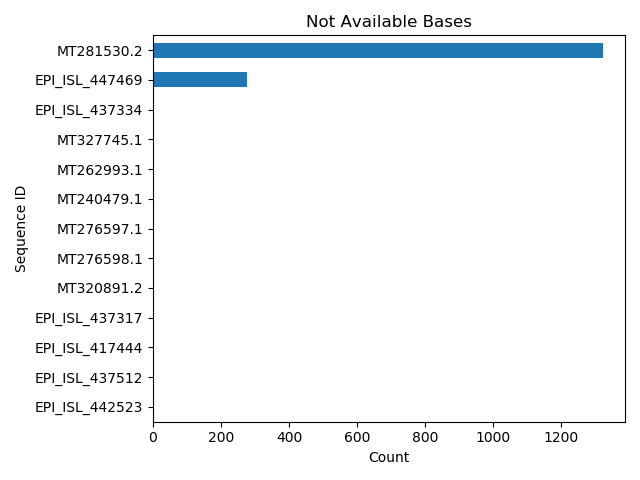
\includegraphics[width=0.9\linewidth]{plot-not-availables.png}}
  \caption{Basi mancanti per sequenza}
  \label{fig:plot-missing}
\end{figure}

\noindent
La \cref{fig:plot-mismatch} presenta, invece, una panoramica sul numero di mismatch per ciascuna sequenza rispetto alla reference di Wuhan. Si nota come le sequenze appartenenti agli stessi paesi risultino avere un numero di variazioni simili ad eccezione della sequenza turca \lstinline{MT327745.1} che presenta un numero più elevato di mismatch e di quella israeliana \lstinline{EPI_ISL_447469}.

Quest'ultima potrebbe discostarsi così tanto dalle altre due sequenze di Israele perché alcune delle variazioni potrebbero risultare nelle porzioni di basi \lstinline{N} identificate precedentemente.

\begin{figure}[H]
  \makebox[\textwidth][c]{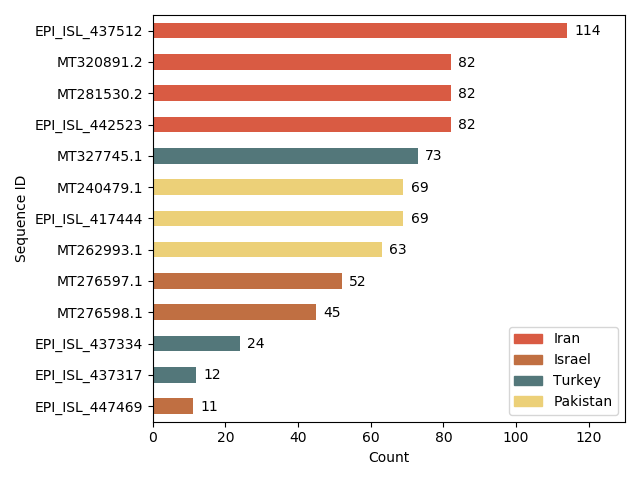
\includegraphics[width=0.8\linewidth]{plot-mismatches.png}}
  \caption{Mismatch rispetto alla sequenza reference}
  \label{fig:plot-mismatch}
\end{figure}

\subsubsection*{Tipologia di variazioni}
Successivamente sono stati considerati i tipi di variazioni rilevati a seconda che questi fossero: cancellazioni, sostituzioni o inserimenti. È possibile notare in \cref{fig:plot-variations-per-type} come quasi 9 variazioni su 10 siano delle cancellazioni di basi rispetto alla reference.

Questo risultato era abbastanza atteso in quanto già dall'analisi preliminare con JalView della sezione \ref{section:pre-analysis}, erano emerse diverse cancellazioni che coinvolgono principalmente l'\textbf{adenina}(\cref{fig:plot-alterations}), infatti la maggior parte delle eliminazioni avvengono agli estremi delle sequenze, dove la reference termina con una serie di 34 adenine.
L'unico inserimento è stato rilevato nella sequenza \lstinline{MT276598.1}(Israele). Tuttavia, come giá mostrato in figura \cref{fig:jalview-start}, questa variazione è prodotta dall'allineamento dei tool e posta prima dell'effettivo inizio rispetto alla sequenza di reference.
\begin{figure}[H]
  \makebox[\textwidth][c]{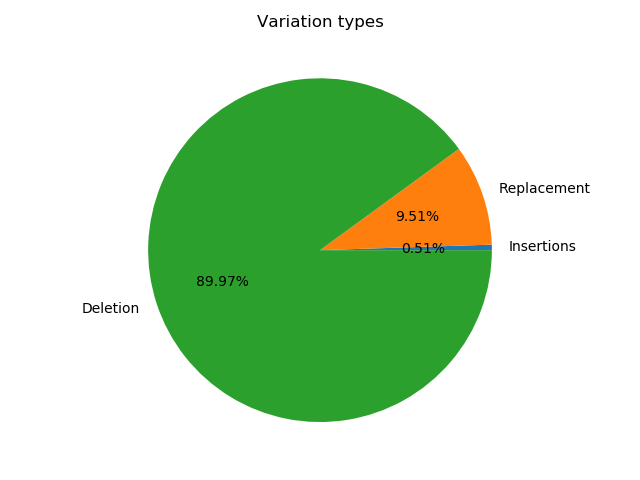
\includegraphics[width=0.85\linewidth]{plot-variations-per-type.png}}
  \caption{Variazioni per tipologia}
  \label{fig:plot-variations-per-type}
\end{figure}

\begin{figure}[H]
  \makebox[\textwidth][c]{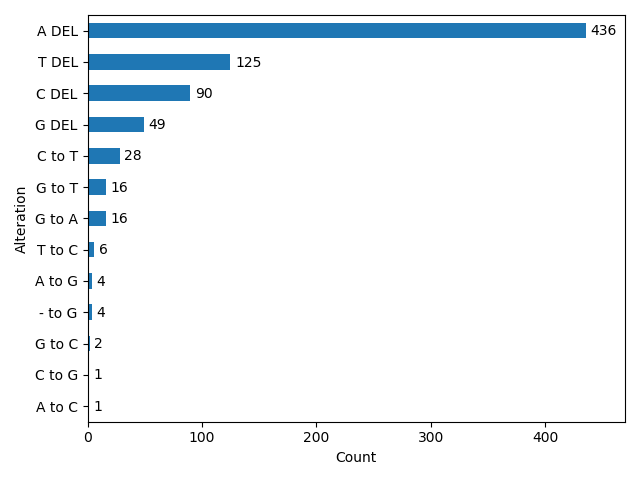
\includegraphics[width=0.85\linewidth]{plot-alterations.png}}
  \caption{Variazioni per tipologia rispetto alle basi coinvolte}
  \label{fig:plot-alterations}
\end{figure}

\noindent
Analizzando ancora più in dettaglio la tipologia di variazioni rispetto alle medesime sequenze (\cref{fig:plot-deletions,fig:plot-replacements}) si nota come cancellazioni e sostituzioni siano distribuite equamente ad eccezione per le sequenze \lstinline{EPI_ISL_437334}(Turchia), \lstinline{EPI_ISL_437317}(Turchia) e \lstinline{EPI_ISL_447469}(Israele) che presentano un numero molto più elevato di sostituzioni. In particolare, la sequenza pakistana \lstinline{MT262993.1} presenta esclusivamente eliminazioni, pur avendo un numero di mismatch omogeneo rispetto alle altre due sequenze dello stesso paese.

\begin{figure}[H]
  \makebox[\textwidth][c]{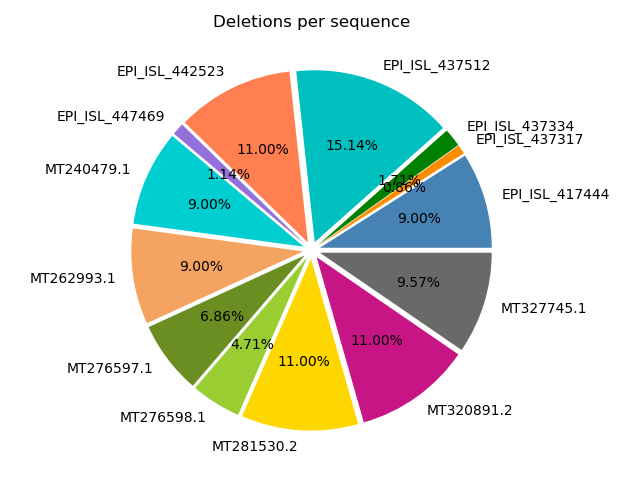
\includegraphics[width=0.65\linewidth]{plot-deletions-per-sequence.png}}
  \caption{Cancellazioni per sequenza}
  \label{fig:plot-deletions}
\end{figure}

\begin{figure}[H]
  \makebox[\textwidth][c]{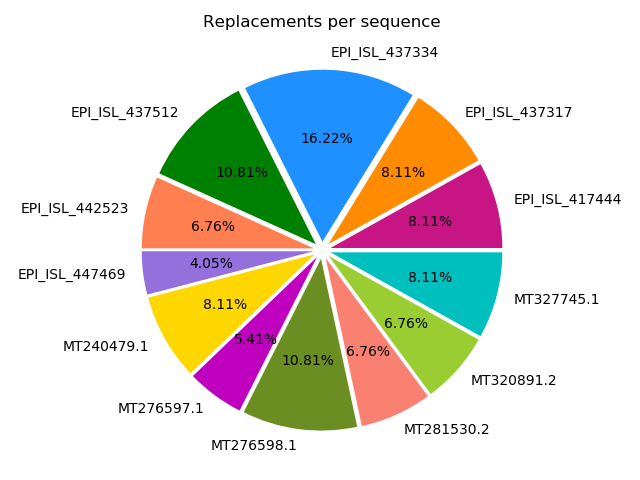
\includegraphics[width=0.65\linewidth]{plot-replacements-per-sequence.png}}
  \caption{Sostituzioni per sequenza}
  \label{fig:plot-replacements}
\end{figure}


\section{Conclusioni}
Dall'analisi preliminare si nota che le sequenze non hanno tutte lo stesso numero di basi, ma la maggior parte dei mismatch si manifesta agli estremi delle sequenze.

Attraverso il confronto degli allineamenti effettuati con Clustal Omega e MUSCLE, la sequenza \lstinline{MT262993.1} è quella che presenta evidenti cancellazioni di più basi contigue che non siano posizionate ai capi della sequenza stessa.
In particolare, sono state rilevate due cancellazioni considerevoli rilevate da entrambi i tool: da \lstinline{9724} a \lstinline{9739}; da \lstinline{19519} a \lstinline{19540}. La sequenza \lstinline{EPI_ISL_437334} pare essere quella con più sostituzioni rispetto al reference; mentre \lstinline{EPI_ISL_437512} è la sequenza con un maggior numero di mismatch complessivi.

Tuttavia, non possiamo determinare se l'incongruenza delle sequenze \lstinline{MT281530.2} e \lstinline{EPI_ISL_437334} rispetto alla reference sia determinata da un'effettiva mutazione piuttosto che da un errore in fase di sequenziamento della stessa.
Le restanti variazioni sporadiche tra le sequenze risultano coinvolgere solamente singole basi.

\subsection{Divisone del lavoro}
Durante la realizzazione del progetto entrambi i componenti del gruppo hanno partecipato attivamente alla sua realizzazione. In particolare:
\begin{itemize}
  \item \textbf{Edoardo Silva} si è occupato principalmente di recuperare le sequenze identificate su NCBI e GISAID e della generazione dei file di output.
  \item \textbf{Davide Marchetti} si è occupato principalmente di scrivere i parser per i tool di allineamento e dell'elaborazione dei gruppi di mismatch per generare il confronto tra i due tool.
  \item Entrambi hanno lavorato all'identificazione dei mismatch tra sequenze sui singoli tool, all'analisi ed elaborazione dei risultati e collaborato alla stesura di questo documento.
\end{itemize}
\end{document}
